\begin{frame}
\frametitle{Audience Poll: Challenges of Parallel Programming}
How many of you have written parallel programs that suffer from:
\begin{itemize}[<+->]
\only<1>{\item Bad scaling?
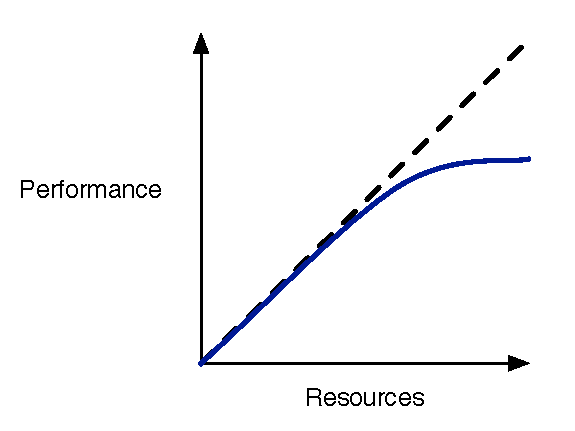
\includegraphics{../figures/bad_scalability.pdf}}
\only<2>{\item Sad scaling?
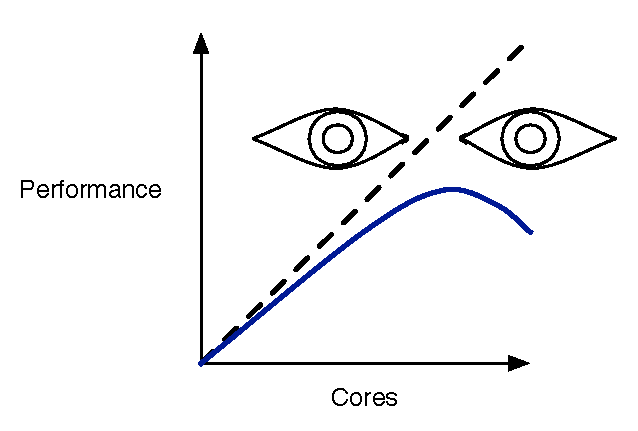
\includegraphics{../figures/sad_scalability.pdf}}
\item Bad scaling?
\item Races, deadlocks, etc: gremlins of shared state?
\pause
\item Limited to shared memory? GPU? No sharing allowed?
\item Coded to match core count?
\only<6>{
\item Independent tasks serialized or badly split across resources?
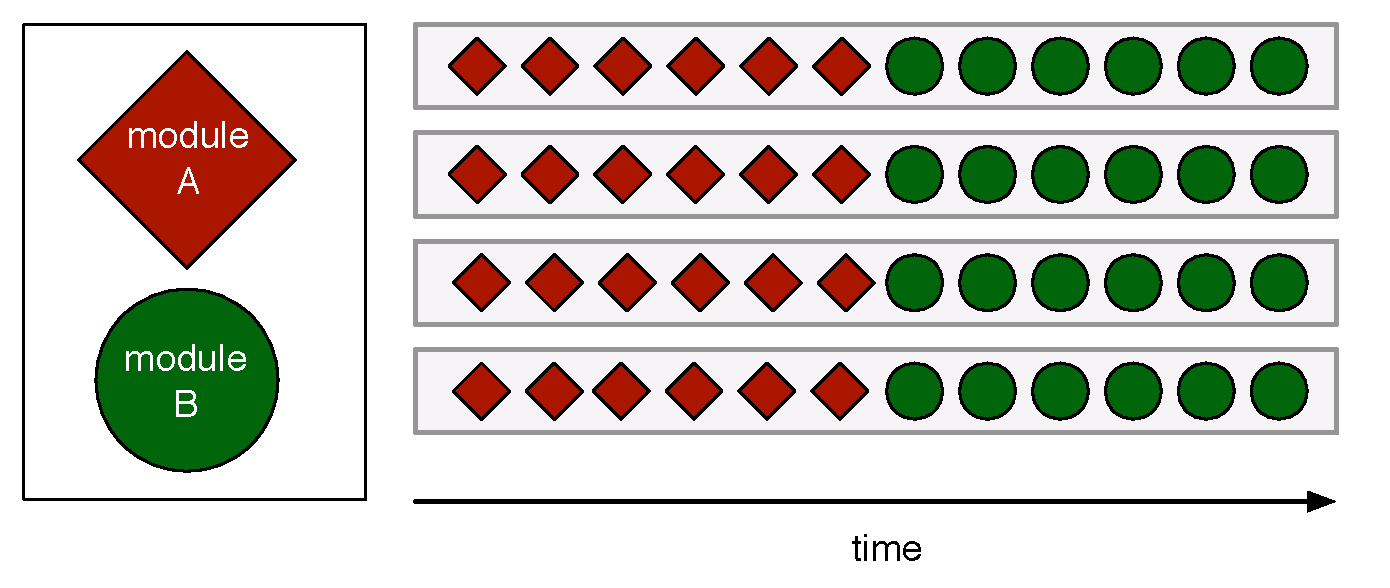
\includegraphics[width=.45\textwidth]{../figures/timeDivision.pdf}\\
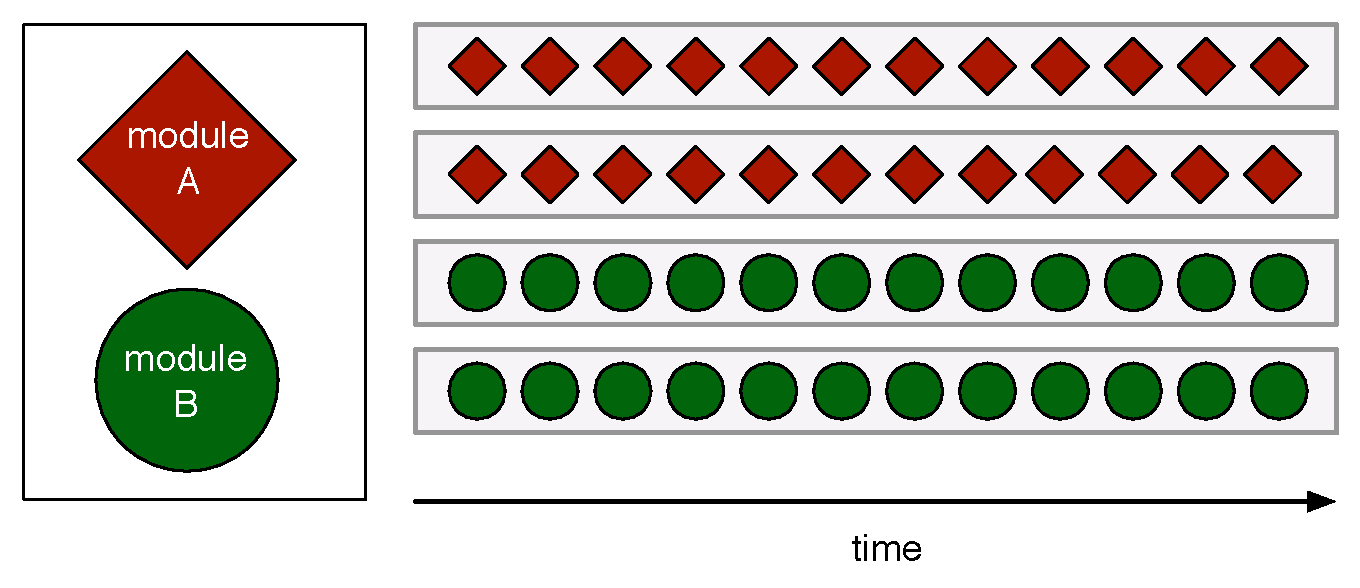
\includegraphics[width=.45\textwidth]{../figures/spaceDivision.pdf}
}
\item Independent tasks serialized or badly split across resources?
\item Application logic interwoven with parallelism optimizations?
\item Wasted energy?
\item Square-peg logic in round-hole framework abstractions?
\end{itemize}
\end{frame}
